\section{Einführung und Grundlagen}
	%TODO@Christian: Aufgabenstellung + EBIS Aufbau und Funktionsweise
    
    \subsection{Aufgabenstellung}
    Eine Elektronenstrahlionenquelle (EBIS) ermöglicht die Herstellung und Entnahme hochgeladener Ionen. Damit ist es möglich, die zeitliche Entwicklung von Ladungszuständen zu beobachten, woraus sich Aussagen über die Ionisationseigenschaften des Elektronenstrahls treffen lassen. \\
    Das Ziel dieses Versuches besteht darin, die Abhängigkeit der Ionisation von Ionisationszeit und Druck in der Ionenquelle zu untersuchen. Dafür werden zunächst die Betriebsparameter der Anlage eingestellt und die Extraktion des Ionenstrahls optimiert.
    Es folgt die Aufnahme eine Übersichtsspektrums der Ionen Ar$^{8+}$ bis Ar$^{18+}$ bei einer gegebenen, festen Ionisationszeit und einem mittleren Arbeitsdruck.
    Mit dem gleichen mittleren Druck wird die Zeitentwicklung der Ionenisationszustände 8+ bis 17+ aufgenommen.
    Danach erfolgt die Messung der Übersichtsspektren bei höherem und niedrigeren Arbeitsdrücken.
    
    \subsection{Aufbau und Funktionsweise des Versuchsplatzes}
        Der Versuch findet an der Microbeam Facility (MBF) statt. Diese ist in Abbildung \ref{aufb} als Draufsicht dargestellt. Sie besteht aus der Electron Beam Ion Source - A (EBIS-A), einer Einzellinse, mehreren Deflektoren, zwei Faraday Cups sowie der Targetkammer. 
        \begin{figure}[htbp]
            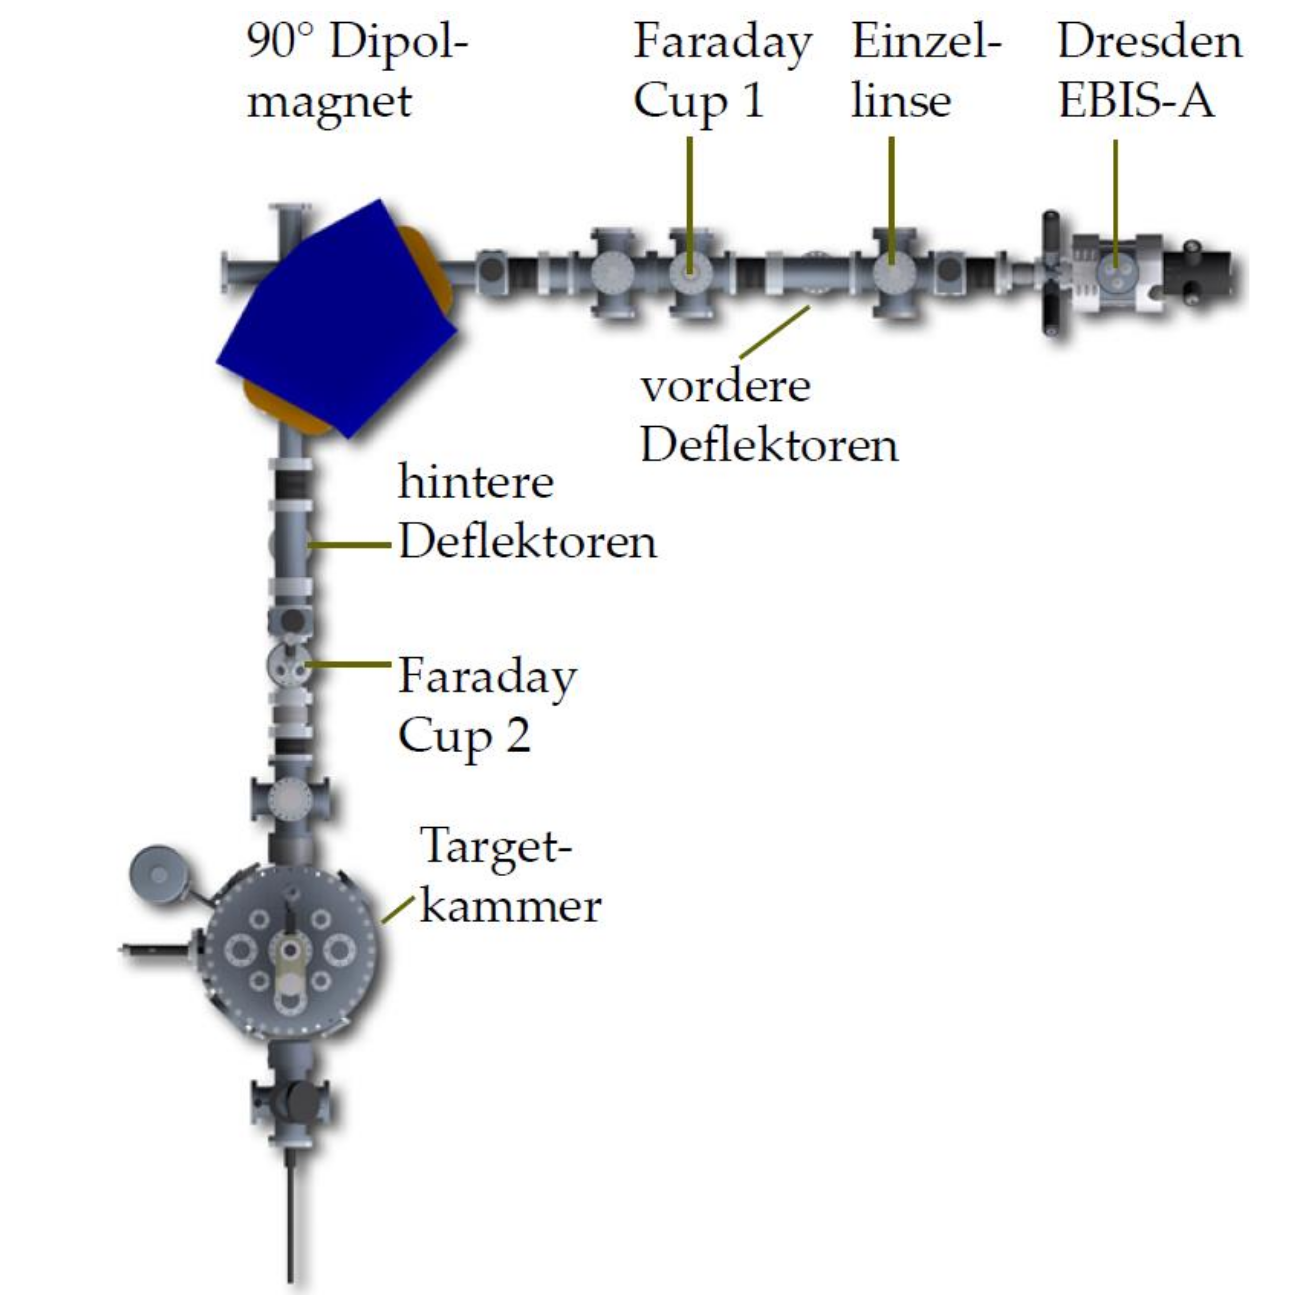
\includegraphics[scale=.8]{pic/aufbau.png}
            \caption{Schematischer Aufbau der MBF, Draufsicht \cite{PA}}
            \label{aufb}
        \end{figure}
        Im Folgenden soll die Funktionsweise der ionenoptischen Komponenten und der EBIS-A kurz erklärt werden.
        Targetkammer wird im Versuch nicht verwendet.
        \subsubsection{Elektronenstrahlionenquelle A}
            In der EBIS-A wird durch eine Elektronen stark emittierende Glühkathode in Zusammenarbeit mit elektrischen Feldern ein Elektronenstrahl erzeugt. Ein äußeres Magnetfeld verdichtet diesen. Der Strahl ionisiert primär neutrale Atome durch Stoßionisation bis sich zwischen Rekombinations- und Ionisationsprozessen ein Gleichgewicht einstellt. Für hohe Ladungszustände müssen die Ionen möglichst lange im Bereich des Elektronenstrahls verweilen. Um dies zu erreichen, besteht zentral aus einer Kombination von Driftröhren, welche eine Zusammenstellung dreier konzentrischer Ringelelektroden sind. 
       \subsubsection{Einzellinse}
           In Abbildung \ref{lense} ist eine Einzelne dargestellt. Sie dient der Fokussierung des Ionenstrahls und ist eine elektrostatische Linse. Sie besteht aus drei zylindrischen Segmenten, wobei das Mittle ein stark negatives Potential besitzt und die beiden anderen auf Erdpotential liegen. Diese Konfiguration erzeugt gekrümmte Äquipotentialflächen, was analog zu einer optischen Linse der Fokussierung entspricht. 
           Variiert man das Potential, das heißt, die anliegende Spannung, so kann die Brennweite justiert werden, was einen Fokus auf die Brennebene ermöglicht.
        \subsubsection{Deflektoren}
            Deflektoren sind schräg eingeschnittene Zylinder, deren Radius orthogonal zur Strahlrichtung steht. Sie liegen parallel zum Strahlkanal und lenken den Ionenstrahl durch elektrostatische Felder ab. Sie sind im Grunde genommen Kondensatoren, welche schiefe und achsenferne Strahlen in Richtung der Strahlachse ablenken können und sich praktisch gut dem zylindrischen Design des Niederenergiestrahlkanals einpassen. In Abbildung \ref{defl} sind zwei Deflektoren (vertikaler und horizontaler) samt ihrer Lage zur Straglrichtung skizziert.
        \subsubsection{Faradaycup}
            Die Faradaycups messen die extrahierten Ionen. Sie sind elektrisch isolierte Metallbecher, welche in den Ionenstrahl gefahren werden, um die Ionen aufzufangen. Ausgelesen wird die eingefallene Ladung über ein Elektrometer oder einen kalibrierten Widerstand. Hierbei können durch Auftreffen von Ionen auf die Becheroberfläche Sekundärelektronen freigesetzt werden, welche die Messergebnisse verfälschen. Um das zu verhindern, wird häufig ein weiteres elektrisches Feld eingesetzt, welches die Elektronen daran hindert, den Becher zu verlassen.  \\
            In Abbildung \ref{cup} ist ein Faradaycup skizziert. 
           
        \begin{figure}[htbp]
            \centering
              \subfigure[Skizze eines Deflektors\label{defl}]{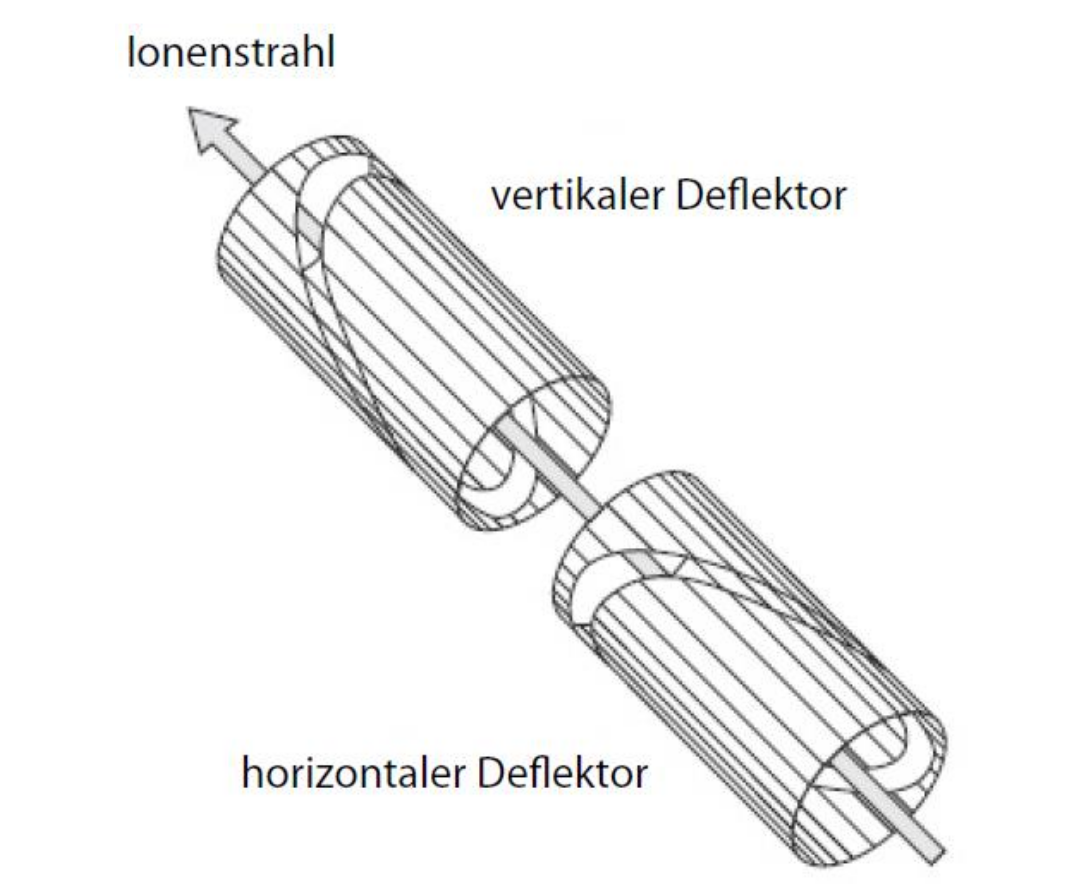
\includegraphics[scale=.35]{pic/deflektor.png}}
              \subfigure[Skizze eines Faradaycups\label{cup}]{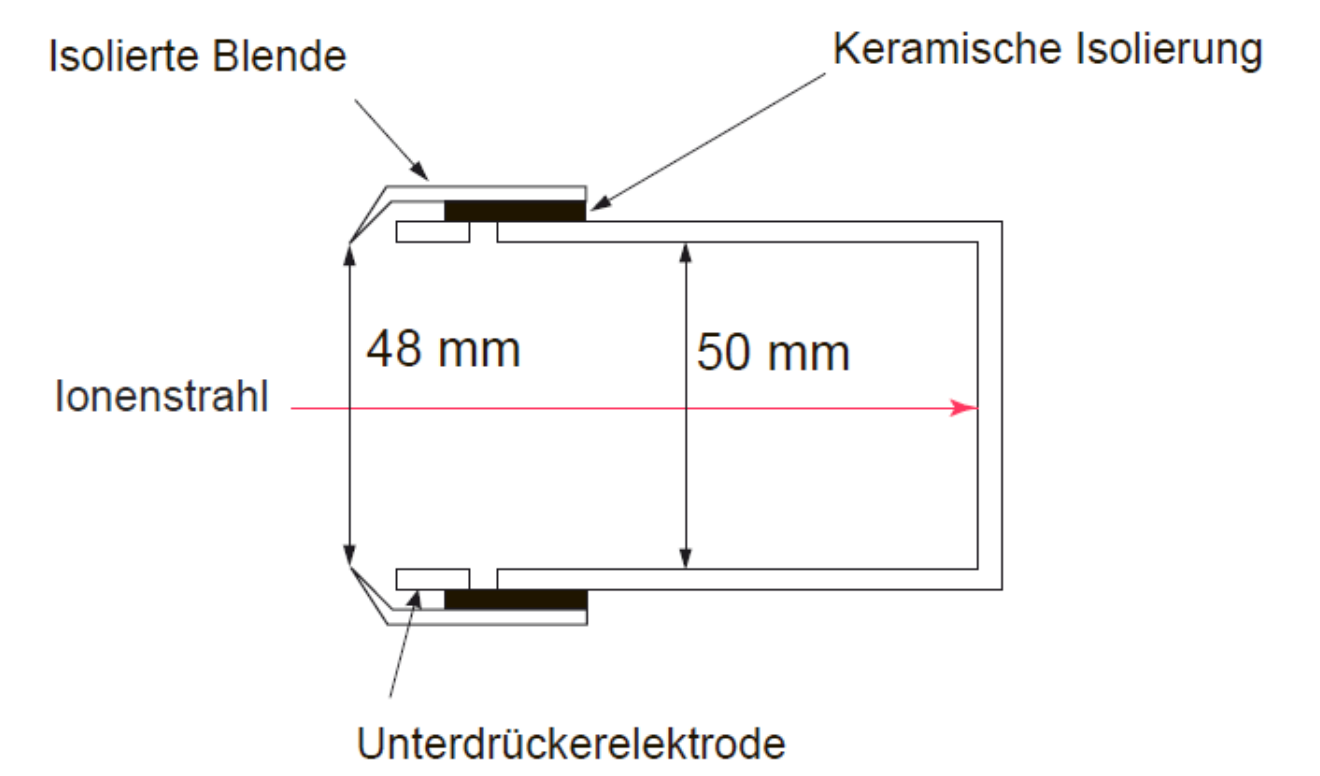
\includegraphics[scale=0.35]{pic/faradaycup.png}}
              \subfigure[Skizze und Schema einer Einzellinse\label{lense}]{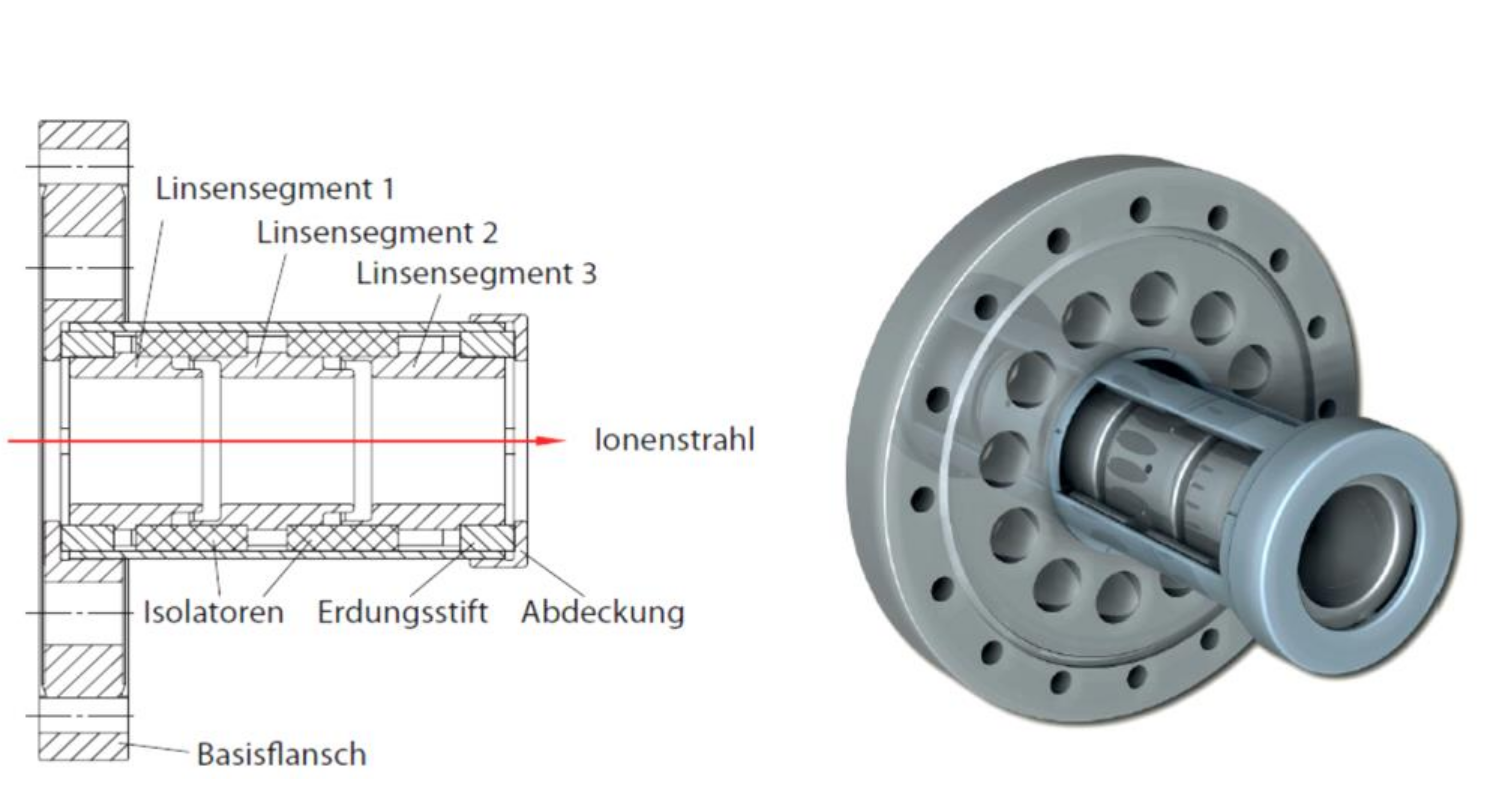
\includegraphics[scale=0.35]{pic/linse.png}}   \caption{Einige Bestandteile der MBS \cite{PA}}
              \label{teile}         
        \end{figure}
	\subsection{Elektrisch geladene Teilchen in einem homogenen Mag\-net\-feld}
		Um später die verschiedenen elektrisch geladenen Argonionen voneinander trennen zu können, ist im Niederenergiestrahlkanal ein 90°-Dipol-Magnet verbaut, der ein homogones Magnetfeld erzeugt und die Ionen auf eine Kreisbahn zwingt. Im Folgenden soll die Dynamik dieser Bewegung erörtert werden.\\
		Betrachte dafür ein elektrisch geladenes Teilchen mit Ladung $Q = q\cdot e$ und Masse $m$. Es wurde vorher von einem elektrischen Feld mit einer Spannung $U_B$ auf die Geschwindigkeit $\vec{v}(t=0)=v\vec{e}_x$ beschleunigt und befinde sich anschließend in einem homogenen Magnetfeld $\vec{B} = B \vec{e}_z$. In diesem erfährt es die \textit{Lorentzkraft}:
		\begin{equation}\label{eq:lorentz}
			\vec{F}_L(t) = Q\cdot\vec{v}(t)\times\vec{B} = QB(-v_x(t) \vec{e}_x + v_y(t)\vec{e}_y) = m\cdot \dot{\vec{v}}(t) \perp \vec{v}(t).
		\end{equation}
		Die z-Komponente ändert sich dabei nicht, somit findet die Bewegung o.B.d.A. in der x-y-Ebene statt. Da die Kraft zusätzlich zu jedem Zeitpunkt $t$ senkrecht zu der Geschwindigkeit ist, entsteht eine Bewegung auf einer Kreisbahn, deren Radius $R$ durch das Kräftegleichgewicht zwischen Lorentzkraft (\ref{eq:lorentz}) und der Zentrifugalkraft(\ref{eq:zentrifugal}) bestimmt wird:
		\begin{align}
			&\vec{F}_Z = - \frac{m\cdot v^2}{R}\cdot \frac{\vec{F}_L}{|\vec{F}_L|} \overset{!}{=} - \vec{F}_L \label{eq:zentrifugal}\\
			&\Rightarrow R = \frac{mv}{QB} = \sqrt{\frac{2U_Bm}{QB^2}}\label{eq:radius}
		\end{align}
		Wobei (\ref{eq:radius}) aus der Ersetzung der Geschwindigkeit durch die Beschleunigungspannung $U_BQ = mv^2/2$ erfolgte. Im Experiment ist der Radius $R = \unit[461]{mm}$ des Dipolmagneten vorgegeben, somit können durch Variation der Magnetflussdichte $B$ Teilchen einer bestimmten spezifischen Ladung $Q/m$ ausgefiltert werden. Dies wird später außerdem dazu genutzt, um Fremdionen im Übersichtsspektrum bei niedrigen Drücken identifizieren zu können, wobei die Zuordnung durch die Verhältnisbildung Masse zu Ladung nicht unbedingt eindeutig ist.
	
	\subsection{Wechselwirkungsprozesse von Ionen} \label{sec:ww}
		Trifft der Elektronenstrahl der EBIS auf die im Potentialtopf gebundenen neutralen Atome, beginnt die sukzessive Ionisation dieser bis sich in der Quelle ein stationärer Zustand zwischen Ionisations- und Rekombinationsprozessen einstellt. Um diesen Vorgang besser zu verstehen, sollen im Folgenden Abschnitt kurz die wichtigsten physikalischen Effekte diskutiert werden.\\
		Der in der Ionenquelle dominante \textbf{Ionisationsvorgang}, ist die sogenannte \textbf{Elektronenstoßionisation}. Dabei wird ein Elektron des Atoms oder Ions aus der Atomhülle durch Zusammenstoß mit einem Elektron des Kathodenstrahls herausgelöst. Die kinetische Energie des Strahlelektrons muss dabei größer sein als die Ionisationsenergie des Atoms.
		\begin{equation}
			\text{X}^{q+} + e^{-} \rightarrow \text{X}^{(q+1)+} + 2e^{-}
		\end{equation}
		Der \textbf{Augerprozess} stellt einen mehrstufigen Ionisationsvorgang dar. Dabei wird ein Atom durch einen Elektronenstoß in einen metastabilen angeregten Zustand versetzt und kehrt unter Aussendung eines sogenannten Augerelektrons eines äußeren Orbitals in den Grundzustand zurück.
		\begin{equation}
					\text{X}^{q+} + e^{-} \rightarrow (\text{X}^{q+})^* + e^{-} \rightarrow \text{X}^{(q+1)+} + 2e^{-}
		\end{equation}
		Prozesse, die der Erhöhung der Ladungszustände von Ionen entgegenwirken, nennt man \textbf{Rekombinationsvorgänge}. Der in der Quelle dominante Prozess dieser Art ist die \textbf{strahlende Rekombination}. Dabei wird ein Elektron aus dem Elektronenstrahl in der Hülle eines Ions eingefangen. Die dabei freiwerdende Bindungsenergie und überschüssige kinetische Energie des Elektrons wird in Form eines Photons emittiert.
		\begin{equation}
			\text{X}^{q+} + e^{-} \rightarrow \text{X}^{(q-1)+} + \hbar\omega
		\end{equation}
		Neben den Wechselwirkungen der Elektronen des Kathodenstrahles mit den Atomen in der Falle kommt es auch zu Interaktionen der Ionen untereinander. Ein Prozess dieser Art ist der \textbf{Ladungsaustausch}, der besonders hoch ionisierte Teilchen bei Zusammenstößen in niedrigere Ladungszustände versetzt. Dabei findet für $q<p$ folgende Reaktion statt:
		\begin{equation}
			X^{q} + X^{p} \rightarrow X^{q+1} + X^{p-1}.
		\end{equation}
		Der Wirkungsquerschnitt für diesen Prozess ist proportional zur Energie der Ionen und nimmt somit für hohe Arbeitsdrücke zu. Will man besonders hohe Ionisationszustände erreichen, ist es somit notwendig, den Druck so gering wie möglich zu halten.\cite{PA}
		